\documentclass[10pt,a4paper]{article}
\usepackage[utf8]{inputenc}
\usepackage{amsmath}
\usepackage{amsfonts}
\usepackage{amssymb}
\usepackage{hyperref}
\usepackage{graphicx}
\graphicspath{ {./images/} }

\author{Andrei Cristian\\\url{mailto:andrei.cristian1@info.uaic.ro}}
\title{Lab 3 - Exercise 4}

\begin{document}
%%%%%%%%%%commands%%%%%%%%%%
\newcommand{\llbracket}{[\![}
\newcommand{\rrbracket}{]\!]}
%%%%%%%%%%commands%%%%%%%%%%
\maketitle
\section{Exercise 6}
For the Labelled Transition System below, compute the following sets of states:

\begin{figure}[ht]
\centering
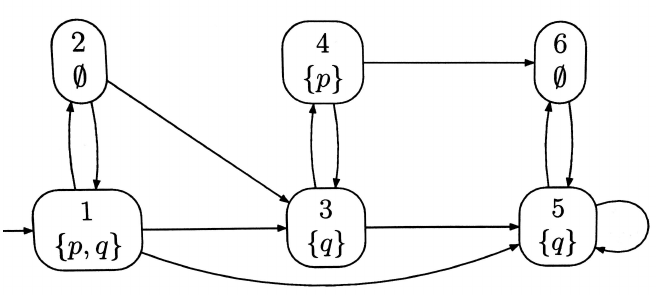
\includegraphics[scale=0.6]{ex4_labelled_transition_system.png}
\end{figure}

\begin{enumerate}
\item $\llbracket EF_p \rrbracket$
\item $\llbracket AF_q \rrbracket$
\item $\llbracket \varphi \rrbracket$, where $\varphi = E( qU (p \wedge \neg q )$
\item $\llbracket \varphi \rrbracket$, where $\varphi = EGq \vee ( EGp \wedge EFq )$
\end{enumerate}

\section{Solving of exercise 6}

\end{document}